\documentclass[11pt]{article}
\usepackage[T1]{fontenc}
\usepackage{lmodern}
\usepackage[margin=1in]{geometry}
\usepackage{amsmath,amssymb,amsthm,mathtools}
\usepackage{booktabs,array}
\usepackage{microtype}
\usepackage{xcolor}
\usepackage{tikz}
\usepackage{flafter}
\usepackage[colorlinks=true,linkcolor=blue!55!black,citecolor=blue!55!black,urlcolor=blue!55!black]{hyperref}
\hypersetup{pdftitle={The Gaussian propeller bound in every dimension},pdfauthor={OpenAI}}
\numberwithin{equation}{section}
\newtheorem{theorem}{Theorem}[section]
\newtheorem{lemma}[theorem]{Lemma}
\newtheorem{proposition}[theorem]{Proposition}
\newtheorem{corollary}[theorem]{Corollary}
\theoremstyle{definition}
\newtheorem{definition}[theorem]{Definition}
\theoremstyle{remark}
\newtheorem{remark}[theorem]{Remark}
\newcommand{\Clust}{\operatorname{Clust}}
\newcommand{\val}{\operatorname{val}}
\newcommand{\OBJ}{\operatorname{OBJ}}
\newcommand{\Inf}{\operatorname{Inf}}
\newcommand{\one}{\mathbf 1}
\newcommand{\E}{\mathbb E}
\newcommand{\R}{\mathbb R}
\newcommand{\Q}{\mathbb Q}
\newcommand{\N}{\mathbb N}
\title{The Gaussian propeller bound in every dimension}
\author{OpenAI}
\date{September 24, 2026}
\begin{document}
\maketitle
\begin{abstract}
We prove the Gaussian propeller conjecture: for every finite measurable
partition of a Euclidean space, the sum of the squared lengths of its
Gaussian first moments is at most $9/(8\pi)$.
For dimension at least two and at least three cells, three planar
sectors of angle $2\pi/3$, extended by an orthogonal Euclidean factor,
attain the bound.
\end{abstract}

\section{Introduction}
\label{sec:introduction}
Let $\gamma_n$ denote the standard Gaussian probability measure on
$\mathbb R^n$, with density
$(2\pi)^{-n/2}\exp(-\|x\|^2/2)$.
For a measurable set $A\subseteq\mathbb R^n$, its Gaussian first moment is
$z(A)=\int_A x\,d\gamma_n(x)$. We call this unnormalized vector its
\emph{centroid}. Thus a centroid is not divided by the measure of its
cell. For positive integers $d,k$ and a measurable partition
$\mathcal A=(A_1,\ldots,A_k)$ of $\mathbb R^d$, define
\[
 \mathcal F(\mathcal A)=\sum_{i=1}^k\|z(A_i)\|^2.
\]
Partitions are understood up to Gaussian null sets, and empty cells are
allowed. The cell probabilities are unrestricted. All norms and inner
products below are Euclidean.

The propeller conjecture asks whether three planar sectors meeting at
angles $2\pi/3$, extended by an orthogonal Euclidean factor, maximize
this functional whenever $d\ge2$ and $k\ge3$. It arose in Khot and
Naor's study of approximate kernel clustering~\cite{KhotNaor}, where
Gaussian first moments govern approximation and Unique Games hardness.
Their formulation uses $k$ cells in $\mathbb R^{k-1}$, with unused
cells permitted. They proved that a maximizer can be chosen to be a
conical partition in the span of its centroids and determined the
three-cell value~\cite[Theorem~1.2 and Corollary~3.4]{KhotNaor}.

Heilman, Jagannath, and Naor proved the bound for every finite partition
of $\mathbb R^3$~\cite[Theorem~1.1]{HJN}. Their computer-assisted
argument treats the remaining four-cell conical configurations through
spherical geometry and a finite verification. We use that theorem as
an established input. The new estimates below show that an extremizer with five or more
active cells cannot have value greater than $9/(8\pi)$. Here an active
cell has positive Gaussian measure. This proves the conjecture in all
remaining dimensions.

\begin{theorem}\label{thm:main}
For all positive integers $d$ and $k$, every measurable partition
$(A_1,\ldots,A_k)$ of $\mathbb R^d$ satisfies
\[
 \sum_{i=1}^k\left\|\int_{A_i}x\,d\gamma_d(x)\right\|^2
 \le\frac9{8\pi}.
\]
Empty cells are allowed. The constant is sharp whenever $d\ge2$ and
$k\ge3$: three planar sectors of angle $2\pi/3$, multiplied by the
orthogonal complement of their plane, attain equality, with any further
cells empty.
\end{theorem}

\subsection{The attaining propeller}
\label{sec:example}
The attaining partition illustrates an important feature of the
problem: in every dimension at least two, only three cells are needed
once at least three labels are available.

Consider a sector $P$ in $\mathbb R^2$ of opening
$2\alpha$, symmetric about the first coordinate axis. Polar integration
gives
\[
 \int_P x\,d\gamma_2(x)
 =\frac1{2\pi}\left(\int_0^\infty r^2e^{-r^2/2}\,dr\right)
      \left(\int_{-\alpha}^{\alpha}(\cos\theta,\sin\theta)\,d\theta\right)
 =\frac{\sin\alpha}{\sqrt{2\pi}}(1,0).
\]
For $\alpha=\pi/3$, three such sectors partition the plane and their
squared centroid lengths sum to
$3\sin^2(\pi/3)/(2\pi)=9/(8\pi)$.
An orthogonal Gaussian factor contributes zero to every centroid, so
the construction has the same value in every dimension at least two.
The construction proves the attainment assertion in
Theorem~\ref{thm:main}.
Figure~\ref{fig:propeller-sectors} shows the planar partition and its
centroid directions.
\begin{figure}[htbp]
  \centering
  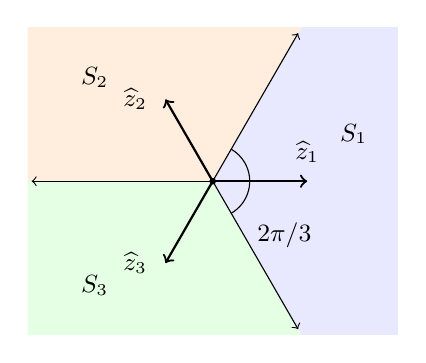
\begin{tikzpicture}[x=1cm,y=1cm,line cap=round,line join=round,
                      font=\small]
    \begin{scope}
      \clip (-2.35,-1.95) rectangle (2.35,1.95);
      \fill[blue!9] (0,0) -- (-60:8) -- (60:8) -- cycle;
      \fill[orange!13] (0,0) -- (60:8) -- (180:8) -- cycle;
      \fill[green!10!white] (0,0) -- (180:8) -- (300:8) -- cycle;
    \end{scope}
    \draw[->,thin] (0,0) -- (60:2.17);
    \draw[->,thin] (0,0) -- (180:2.30);
    \draw[->,thin] (0,0) -- (300:2.17);
    \draw[thick,->] (0,0) -- (0:1.20)
      node[above=3pt] {$\widehat z_1$};
    \draw[thick,->] (0,0) -- (120:1.20)
      node[left=3pt] {$\widehat z_2$};
    \draw[thick,->] (0,0) -- (240:1.20)
      node[left=3pt] {$\widehat z_3$};
    \draw[thin] (-60:.47) arc[start angle=-60,end angle=60,radius=.47];
    \node at (.91,-.69) {$2\pi/3$};
    \node at (1.79,.60) {$S_1$};
    \node at (-1.50,1.32) {$S_2$};
    \node at (-1.50,-1.32) {$S_3$};
    \fill (0,0) circle[radius=1.2pt];
  \end{tikzpicture}
  \caption{The attaining planar partition consists of three unbounded
  sectors $S_1,S_2,S_3$ of angle $2\pi/3$; only a finite window is shown.
  The bold arrows show the unit centroid directions
  $\widehat z_i=z(S_i)/\|z(S_i)\|$.
  Each unnormalized Gaussian centroid has length
  $\sqrt{3}/(2\sqrt{2\pi})$, so their squared lengths sum to
  $9/(8\pi)$. In dimension $d\ge2$, use
  $S_i\times\mathbb R^{d-2}$, with any further cells empty.}
  \label{fig:propeller-sectors}
\end{figure}



\subsection{Analytic background and related partition problems}
The geometric reduction in Khot and Naor's work is also the starting
point here. We reprove its needed form, including attainment, the
maximal-score description of the cells, and the effective dimension.
The Gaussian-maximum duality used in this reduction is the normalized
vector form of their Lemma~3.7. Our estimates then combine the loss on deleting
one score with bounds for competition against two residual scores.

The one-score estimate uses the Gaussian Minkowski inequality introduced
by Ehrhard for convex sets~\cite{Ehrhard}. Lata\l a extended the
inequality when one of the sets is convex~\cite{Latala}; Borell proved
the Borel-set version~\cite[Theorem~1.1]{Borell}. Van Handel later gave
a stochastic-game proof~\cite{vanHandel}. We need only the convex case:
applied to translates of a cell, the inequality makes its inverse-normal
Gaussian measure a concave function of the translation parameter. The
translation direction, derivative, and resulting deletion estimate are
derived in Section~\ref{sc:section}.

A related question asks which partition maximizes the probability that
two correlated Gaussian vectors belong to the same cell, often with
equal cell probabilities prescribed. This noise-stability objective
is distinct from the unrestricted first-moment functional studied here.
Heilman~\cite[Theorem~1.7]{HeilmanHyper} obtained a conditional route to
the propeller bound for three or four cells in arbitrary dimension,
assuming an additional stability property of equal-volume
noise-stability maximizers. That result retains both the stability
hypothesis and the restriction to at most four cells. The present
argument addresses all finite cell counts and imposes no cell-mass
constraint.

\subsection{The kernel-clustering consequence}
The Gaussian constant also determines the identity-target
kernel-clustering threshold. For a rational symmetric positive
semidefinite matrix $A=(a_{pq})_{p,q=1}^N$ with $A\one=0$, this problem
asks for an assignment $\sigma:[N]\to[k]$ maximizing
\[
 \sum_{p,q=1}^N a_{pq}\one_{\{\sigma(p)=\sigma(q)\}}.
\]
Here $[N]=\{1,\ldots,N\}$, $\one$ is the all-ones vector, and the
indicator is one when its subscripts have the same label. Empty
clusters are allowed. A loss factor $\alpha$ means returning an
assignment worth at least $1/\alpha$ times the maximum value.
For fixed $k\ge3$, Khot and Naor's expected Gaussian rounding guarantee
\cite[Theorem~2.1]{KhotNaor} has loss factor
\[
 \alpha_k=\frac{8\pi}{9}\left(1-\frac1k\right).
\]
Theorem~\ref{thm:main} evaluates the Gaussian partition parameter in
their hardness analysis. Together with their low-influence theorem and
the companion paper \emph{The Unique Games Theorem}
\cite[Theorem~1.1]{UniqueGamesTheorem}, it gives NP-hardness of every
deterministic approximation with a fixed loss factor below $\alpha_k$.
Section~\ref{kc:section} proves this application on rational inputs and
specifies the ideal rounding convention at the endpoint. The separate
Unique Games input is needed only for the hardness statement.

\subsection{Proof strategy}
The difficulty is to control all measurable partitions while allowing
both their shapes and their probabilities to vary. We first replace
this infinite-dimensional optimization by a finite list of Gaussian
linear scores. Two different consequences of optimality then constrain
that list: deleting one score costs a definite amount of expected
maximum, and competing against two scores constrains a covariance
determinant.

Section~\ref{ext:section} proves the reduction in full. Norm duality
identifies the square root of the largest possible partition value
with the largest possible expectation of the maximum score over lists
of vectors with total squared norm one. Compactness gives an extremizer. Among extremizers, choose
one with the fewest cells of positive measure. Merging two cells shows
that its nonzero centroids $z_1,\ldots,z_m$ have strictly negative
pairwise inner products. Its cells agree almost everywhere with the
cones where the corresponding score $\langle z_i,x\rangle$ is largest.
The centroids span a space of dimension $m-1$. The theorem of
Heilman, Jagannath, and Naor therefore excludes $m\le4$ from any
counterexample to the desired bound.

For the remaining case $m\ge5$, let $C$ be the optimal value, let
$r_i=\|z_i\|/\sqrt C$ be the normalized centroid lengths, and let
$P_i$ be the cell probabilities. Then $\sum_i r_i^2=\sum_iP_i=1$.
Section~\ref{sc:section} bounds each $P_i$ below in terms of $r_i$.
Halfspace rearrangement gives one such estimate; when $m=5$, spherical
rearrangement in the four-dimensional centroid span improves it.
A further bound comes from removing one score and recentering the
remaining vectors. The extremal score inequality gives a lower bound
for the loss. Translations of the deleted score's winning cone,
together with Ehrhard's inequality, give an upper bound. Comparing the
two produces a scalar constraint on $P_i$ and $r_i$.

Section~\ref{geo:section} uses the cell with the smallest normalized
centroid length. Projecting the other scores orthogonally to its centroid gives
residual Gaussian scores independent of the score in that direction.
Their integrals over the chosen cell vanish. For two residual scores,
these identities allow us to estimate a positive-part integral by
replacing the joint density with its maximum. The denominator of this
two-dimensional Gaussian density bound is the
square root of the residual covariance determinant. The resulting
pairwise bound yields two inequalities involving the three largest
normalized centroid lengths and the smallest one.

Finally, Section~\ref{elim:section} combines the scalar probability
bounds with the identity $\sum_iP_i=1$. The available probability mass
forces the third-largest squared length to be too large relative to
the smallest length, contradicting the determinant bound. This excludes
an optimal value above $9/(8\pi)$. Appendix~\ref{cert:arithmetic}
gives exact rational enclosures for every finite numerical comparison,
including the complete interval cover needed for the scalar constraint.
The geometric proof uses the three-dimensional propeller bound and
Ehrhard's inequality as its external theorem inputs; the remaining
geometric estimates are proved here. Section~\ref{kc:section} gives a
separate kernel-clustering application. Its reduction adapts Khot and
Naor's construction and uses two additional theorem inputs: their
discrete Fourier estimate and the separate Unique Games theorem in
\cite{UniqueGamesTheorem}.

\section{Extremal partitions and their centroids}
\label{ext:section}

Our goal is to replace an arbitrary measurable partition by an optimal
partition described by finitely many Gaussian linear scores. We include
the extremal reduction of Khot and
Naor~\cite[Theorem~1.2 and Lemma~3.3]{KhotNaor} in the form needed below.

It suffices to prove the upper bound for $n+1$ cells in
$\mathbb R^n$ with $n\ge4$. Indeed, given $k$ cells in
$\mathbb R^d$, put $n=\max\{d,k-1,4\}$, take their products with
$\mathbb R^{n-d}$, and append $n+1-k$ empty cells. Gaussian product
decomposition appends zero coordinates to each first moment and
preserves the objective.

Fix such an $n$ and put $N=n+1$. All partitions below are measurable
partitions up to Gaussian null sets, and empty cells are permitted. Write
\[
 C=\sup_{(A_1,\ldots,A_N)}
       \sum_{i=1}^N\left\|\int_{A_i}x\,d\gamma_n(x)\right\|^2,
 \qquad B=\frac{3}{2\sqrt{2\pi}}.
\]
The moments exist, and Cauchy--Schwarz on each cell gives $C\le n$.
We first record the normalized vector form of the Gaussian-maximum
description in \cite[Lemma~3.7]{KhotNaor}. Its proof also gives
attainment directly.

\begin{lemma}\label{ext:duality}
If $g$ is a standard Gaussian vector in $\mathbb R^n$, then
\begin{equation}\label{ext:dual-formula}
 \sqrt C=
 \max_{\sum_{i=1}^N\|v_i\|^2=1}
       \mathbb E\max_{1\le i\le N}\langle v_i,g\rangle.
\end{equation}
The supremum defining $C$ is attained. Moreover, for every $1\le k\le N$
and every list $v_1,\ldots,v_k\in\mathbb R^n$,
\begin{equation}\label{ext:shorter-list}
 \mathbb E\max_{1\le i\le k}\langle v_i,g\rangle
 \le \sqrt C\left(\sum_{i=1}^k\|v_i\|^2\right)^{1/2}.
\end{equation}
\end{lemma}

\begin{proof}
For a partition with moments $z_i=\int_{A_i}x\,d\gamma_n(x)$,
Euclidean norm duality gives
\[
 \left(\sum_i\|z_i\|^2\right)^{1/2}
 =\max_{\sum_i\|v_i\|^2=1}
       \sum_i\int_{A_i}\langle v_i,x\rangle\,d\gamma_n(x).
\]
Taking the supremum jointly over partitions and lists, and then first
over partitions, yields the right side of \eqref{ext:dual-formula}.
Indeed, for each fixed list the pointwise maximum is attained by assigning
$x$ to a largest score $\langle v_i,x\rangle$, with ties resolved by the
smallest index. This gives a measurable partition. The expected maximum
is continuous in the list: the absolute difference of two maxima is at
most $\|g\|\max_i\|v_i-w_i\|$. Compactness of the sphere of lists therefore
gives a maximizing list. Its score partition has moment norm at least
its pairing with that list, namely $\sqrt C$, so it attains $C$.

For \eqref{ext:shorter-list}, let $Q_1,\ldots,Q_k$ be a score partition
for the specified list, and put $b_i=\int_{Q_i}x\,d\gamma_n(x)$.
Appending $N-k$ empty cells shows that $\sum_i\|b_i\|^2\le C$.
Consequently
\[
 \mathbb E\max_i\langle v_i,g\rangle
 =\sum_i\langle v_i,b_i\rangle
 \le\left(\sum_i\|v_i\|^2\right)^{1/2}
      \left(\sum_i\|b_i\|^2\right)^{1/2},
\]
which proves the assertion.
\end{proof}

We argue by contradiction and henceforth assume
\begin{equation}\label{ext:contradiction}
 C>B^2=\frac{9}{8\pi}.
\end{equation}
Choose an optimal partition with the fewest cells of positive measure,
discard its null cells, and call the remaining cells \emph{active}.
Denote their moments by
$z_1,\ldots,z_m$. Thus
\begin{equation}\label{ext:centroid-identities}
 \sum_{i=1}^m z_i=0,
 \qquad \sum_{i=1}^m\|z_i\|^2=C.
\end{equation}

The following structure statement develops the minimal-cell reduction
of \cite[Lemma~3.3]{KhotNaor}; the rank assertions are proved directly
from the Gram matrix.

\begin{lemma}\label{ext:structure}
The centroids satisfy $\langle z_i,z_j\rangle<0$ for $i\ne j$.
Their span $V$ has dimension $m-1$, every proper subset of the centroids
is linearly independent, and, for each fixed $i$, the $m-1$ vectors
$z_i-z_j$, $j\ne i$, form a basis of $V$.
The optimal cells have the closed conical representatives
\begin{equation}\label{ext:cones}
 K_i=\{x\in\mathbb R^n:
          \langle z_i-z_j,x\rangle\ge0\text{ for every }j\ne i\}.
\end{equation}
Furthermore, $m\ge5$.
\end{lemma}

\begin{proof}
Since $C>0$, we have $m\ge2$. Merging two cells changes the objective by
$2\langle z_i,z_j\rangle$. A positive product would contradict optimality;
a zero product would contradict minimality of $m$. Thus every such
product is negative, and in particular every $z_i$ is nonzero.

For the original optimal partition, pairing each cell with its own
centroid gives
\[
 C\le\mathbb E\max_i\langle z_i,g\rangle\le C,
\]
where the second inequality is \eqref{ext:shorter-list}.
The difference between the maximum score and the assigned score is
nonnegative and has zero integral, so it vanishes almost everywhere.
The centroids are distinct, and their score ties lie on finitely many
Gaussian-null hyperplanes. This proves \eqref{ext:cones}; overlaps
between these closed representatives are immaterial.

Let $Q=(\langle z_i,z_j\rangle)_{i,j=1}^m$ be the Gram matrix.
Its row sums vanish by \eqref{ext:centroid-identities}. Hence, for every
$a=(a_1,\ldots,a_m)\in\mathbb R^m$,
\begin{equation}\label{ext:laplacian}
 a^{\mathsf T}Qa
 =\sum_{i<j}(-\langle z_i,z_j\rangle)(a_i-a_j)^2.
\end{equation}
All weights are positive, so the kernel of $Q$ consists exactly of
constant vectors. Its rank is $m-1$, and the only linear relations among
the centroids are multiples of their sum. A dependence on a proper
subset would have a zero coefficient and therefore must be trivial.
A relation among $z_i-z_j$, $j\ne i$, gives a relation among all centroids
whose coefficients sum to zero; it too must be trivial. This proves
the linear-algebra assertions.

Each $K_i$ depends only on the orthogonal projection onto $V$.
If $d=\dim V$, then orthogonal Gaussian product decomposition identifies
$K_i$ with $(K_i\cap V)\times V^\perp$, and its moment is the moment of
$K_i\cap V$ in $V$, extended by zero on $V^\perp$.
If $m\le4$, then $d\le3$. Taking the product of this partition of
$V\cong\mathbb R^d$ with $\mathbb R^{3-d}$ preserves its moment norms.
The three-dimensional propeller theorem of Heilman, Jagannath, and
Naor~\cite[Theorem~1.1]{HJN}, which permits any finite number of cells,
would then give $C\le9/(8\pi)$, contradicting
\eqref{ext:contradiction}. Thus $m\ge5$.
\end{proof}

We have reduced a hypothetical counterexample to at least five active
cells whose centroid span has dimension one less than their number.
From now on we work in $V\cong\mathbb R^{m-1}$, use $K_i$ for the reduced
cones, and let $g$ be standard Gaussian in this space. Their moments
remain exactly $z_i$. Inequality~\eqref{ext:shorter-list} remains valid
for lists in $V$, by embedding them in $\mathbb R^n$. Set
\begin{equation}\label{ext:notation}
 X_i=\langle z_i,g\rangle,
 \qquad P_i=\gamma_{m-1}(K_i),
 \qquad r_i=\frac{\|z_i\|}{\sqrt C}.
\end{equation}
Then $P_i>0$, $r_i>0$, $\sum_iP_i=\sum_i r_i^2=1$, and
$\mathbb E\max_iX_i=C$. Since $\sum_iX_i=0$, a winning score is
nonnegative. Thus $K_i\subseteq\{X_i\ge0\}$ and
\begin{equation}\label{ext:half-probability}
 P_i\le\frac12\qquad(1\le i\le m).
\end{equation}

\section{Probability bounds for the cells}\label{sc:section}
Throughout this section, we work with the putative extremizer above:
\(C>B^2\), \(m\ge5\), and \(B=3/(2\sqrt{2\pi})\).
We will obtain lower bounds for each cell probability in terms of its
normalized centroid length. Since the probabilities sum to one, these
bounds constrain how the normalized centroid lengths can be
distributed among the cells.
Every terminating decimal in the proof denotes an exact rational number.
Write
\[
 \phi(x)=\frac{e^{-x^2/2}}{\sqrt{2\pi}},\qquad
 \Phi(x)=\int_{-\infty}^x\phi(u)\,du,\qquad
 r_i=\frac{|z_i|}{\sqrt C},\qquad P_i=\gamma_{m-1}(K_i).
\]
The winning cone \(K_i\) lies in \(\{x:\langle z_i,x\rangle\ge0\}\),
because the scores sum to zero. Thus \(0<P_i\le1/2\).

\begin{lemma}\label{sc:bounds}
Set
\[
 A=\begin{cases}0.929,&m=5,\\0.884,&m\ge6.\end{cases}
\]
For every \(i\),
\begin{equation}\label{sc:three-bounds}
 r_i\le\frac23,\qquad P_i\ge Ar_i^2,\qquad
 P_i\ge0.415r_i+0.15r_i^2.
\end{equation}
\end{lemma}

\subsection{Rearrangement bounds}
Fix a cell, and temporarily suppress its index.
Let \(e=z/|z|\), \(x=\Phi^{-1}(1-P)\), and
\(H=\{g:\langle e,g\rangle\ge x\}\). Since \(\gamma_{m-1}(H)=P\),
\[
 |z|-\int_H\langle e,g\rangle\,d\gamma_{m-1}(g)
 =\int(\langle e,g\rangle-x)(1_K-1_H)\,d\gamma_{m-1}(g)\le0.
\]
Consequently \(|z|\le\phi(x)\). As \(\sqrt C>B=(3/2)\phi(0)\),
this proves \(r<2/3\) and
\begin{equation}\label{sc:halfspace-ratio}
 \frac P{r^2}\ge \frac94 e^{x^2}\Phi(-x).
\end{equation}
For completeness, the minimum on the right can be localized by a
one-dimensional argument. Put \(M(x)=\phi(x)/\Phi(-x)\).
The logarithmic derivative of \(f(x)=(9/4)e^{x^2}\Phi(-x)\) is
\(2x-M(x)\), and
\[
 M'(x)=1-\operatorname{Var}(Z\mid Z>x)<1
\]
for a standard normal variable \(Z\). Hence \((\log f)'\) is strictly
increasing. Its signs at \(0.6119\) and \(0.6121\) are opposite, so
\(f\) has a unique global minimum in that interval.
The elementary bounds in Appendix~\ref{cert:arithmetic} give
\begin{equation}\label{sc:halfspace-minimum}
 \min_{x\in\mathbb R}f(x)>0.8843837>0.884.
\end{equation}
This proves the required quadratic estimate when \(m\ge6\).

When \(m=5\), conicality improves the estimate. Work in the
four-dimensional span of the centroids and write the standard Gaussian
as \(RU\), where \(U\) is uniform on \(S^3\) and independent of \(R\).
The coordinate \(\langle e,U\rangle\) has density
\((2/\pi)\sqrt{1-u^2}\) on \([-1,1]\). The same threshold comparison as
above shows that, among spherical sets of measure \(P\), an upper cap
maximizes the first moment in direction \(e\). Since \(P\le1/2\), write
its threshold as \(x\in[0,1)\). Its probability is
\[
 p(x)=\frac12-\frac{\arcsin x+x\sqrt{1-x^2}}\pi.
\]
Using \(\mathbb ER=3\sqrt{2\pi}/4\), its Gaussian first moment is
\[
 \mathbb ER\,\frac2\pi\int_x^1 u\sqrt{1-u^2}\,du
 =\phi(0)(1-x^2)^{3/2}.
\]
It follows that
\begin{equation}\label{sc:cap-ratio}
 \frac P{r^2}\ge R(x):=\frac94\frac{p(x)}{(1-x^2)^3}.
\end{equation}
To identify the global minimum, define
\[
 F(x)=6xp(x)-\frac2\pi(1-x^2)^{3/2},\qquad
 H(x)=p(x)-\frac x\pi\sqrt{1-x^2}.
\]
Direct differentiation gives
\[
 R'(x)=\frac94\frac{F(x)}{(1-x^2)^4},\qquad
 F'(x)=6H(x),\qquad
 H'(x)=\frac{4x^2-3}{\pi\sqrt{1-x^2}}.
\]
Thus \(H\) first decreases and then increases. Since \(H(0)=1/2\)
and \(H(1)=0\), it has exactly one zero in \((0,1)\); it is negative
after that zero. Accordingly \(F\) first increases and then decreases
to \(F(1)=0\). The certified signs \(F(0.29)<0<F(0.294)\) show that
\(F\) has exactly one interior zero and that this zero lies in
\((0.29,0.294)\). It is the unique minimizer of \(R\).
Appendix~\ref{cert:arithmetic} gives \(R(0.29)>0.9312526\) and
\(|R'|<0.03\) on this interval, whence
\begin{equation}\label{sc:cap-minimum}
 \min_{0\le x<1}R(x)>0.9311326>0.929.
\end{equation}
The first two assertions of Lemma~\ref{sc:bounds} follow.

\subsection{The loss on removing one score}
Rearrangement has supplied the radius bound and the quadratic
probability bound. To obtain the remaining linear--quadratic estimate
in Lemma~\ref{sc:bounds}, we use the behavior of the
winning probability under translation. Fix \(i\), put
\(X_j=\langle z_j,g\rangle\), and set \(\alpha=m/(m-1)\).
Removing \(z_i\) and recentering the remaining vectors produces
\(z_j+z_i/(m-1)\), \(j\ne i\), whose squared norms sum to
\(C-\alpha|z_i|^2\). A common translation of the scores has zero
expectation. The extremal dual bound therefore gives
\[
 \mathbb E\max_{j\ne i}X_j\le
 \sqrt C\sqrt{C-\alpha|z_i|^2}.
\]
Since \(\mathbb E\max_jX_j=C\), the loss satisfies
\begin{equation}\label{sc:loss-lower}
 \mathbb E\bigl(X_i-\max_{j\ne i}X_j\bigr)_+
 \ge C\bigl(1-\sqrt{1-\alpha r_i^2}\bigr).
\end{equation}
Here \(u_+=\max(u,0)\).

The vectors \(z_i-z_j\), \(j\ne i\), form a basis of the centroid
span. There is therefore a vector \(h\) in that span satisfying
\(\langle h,z_i-z_j\rangle=1\) for every \(j\ne i\).
For \(u\ge0\), the gap probability is
\[
 p_i(u):=\Pr\{X_i\ge X_j+u\text{ for all }j\ne i\}
       =\gamma_{m-1}(K_i+uh).
\]
Summing the equations defining \(h\) gives
\(\langle h,z_i\rangle=(m-1)/m=1/\alpha\).
Differentiation of the translated Gaussian density, justified by
Gaussian integrability, yields
\begin{equation}\label{sc:translation-derivative}
 p_i'(0)=-\int_{K_i}\langle h,x\rangle\,d\gamma_{m-1}(x)
        =-\langle h,z_i\rangle=-\frac1\alpha.
\end{equation}

Ehrhard's inequality states that \(\Phi^{-1}\circ\gamma_{m-1}\) is
concave under Minkowski interpolation of convex sets
\cite{Ehrhard}; we use the formulation in
\cite[Theorem~1.1]{Borell}, which also allows general Borel sets.
The cone \(K_i\) is closed and convex. Its score-difference normals
form a basis, so it has nonempty interior and is a proper subset of
the centroid span. Minkowski interpolation of two translates of \(K_i\) is the translate
with the interpolated displacement. Hence
\(u\mapsto\Phi^{-1}(p_i(u))\) is concave. All finite translates
have measure strictly between zero and one, and the derivative at
zero exists by \eqref{sc:translation-derivative}. With
\(q=\Phi^{-1}(P_i)\), the supporting tangent gives
\[
 p_i(u)\le\Phi\!\left(q-\frac{u}{\alpha\phi(q)}\right)
 \qquad(u\ge0).
\]
Integration, using \((q\Phi(q)+\phi(q))'=\Phi(q)\), gives
\begin{equation}\label{sc:loss-upper}
 \mathbb E\bigl(X_i-\max_{j\ne i}X_j\bigr)_+
 =\int_0^\infty p_i(u)\,du
 \le\alpha\phi(q)\bigl(q\Phi(q)+\phi(q)\bigr).
\end{equation}
Define
\[
 G(q)=\frac{\phi(q)\bigl(q\Phi(q)+\phi(q)\bigr)}{\Phi(q)^2}.
\]
Combining \eqref{sc:loss-lower} and \eqref{sc:loss-upper}, rationalizing,
and canceling \(\alpha\), we obtain
\begin{equation}\label{sc:loss-constraint}
 P_i^2G\bigl(\Phi^{-1}(P_i)\bigr)
 \ge\frac{Cr_i^2}{1+\sqrt{1-\alpha r_i^2}}
 \ge\frac{B^2r_i^2}{1+\sqrt{1-r_i^2}}.
\end{equation}

\subsection{A linear--quadratic probability bound}
The loss constraint is implicit in the cell probability. To extract
an explicit lower bound, we first prove two monotonicity properties
of \(G\).
\begin{lemma}\label{sc:truncated-variance}
The function \(G\) is nonincreasing and satisfies \(0<G(q)<1\).
Moreover,
\[
 P\longmapsto P^2G\bigl(\Phi^{-1}(P)\bigr)
\]
is increasing on \((0,1/2]\).
\end{lemma}
\begin{proof}
Put \(\lambda=\phi(q)/\Phi(q)\). Integration of the normal density gives
\[
 \mathbb E(Z\mid Z\le q)=-\lambda,\qquad
 V(q):=\operatorname{Var}(Z\mid Z\le q)=1-q\lambda-\lambda^2.
\]
Thus \(G=1-V=\lambda(q+\lambda)\). The distance
\(U=q-Z\), under this conditioning, has positive mean
\(q+\lambda\) and positive variance, proving \(0<G<1\).
Its survival function is
\(S(u)=\Phi(q-u)/\Phi(q)\), \(u\ge0\).
The identity
\((\log\Phi)''(q)=-\lambda(q+\lambda)<0\)
shows that \(\log S\) is concave. Its increments therefore satisfy
\[
 \log S(u+v)-\log S(u)\le\log S(v)-\log S(0).
\]
Since \(S(0)=1\), this gives \(S(u+v)\le S(u)S(v)\).
Integrating over \(u,v\ge0\) gives
\[
 \frac12\mathbb EU^2
 =\int_0^\infty\!\int_0^\infty S(u+v)\,du\,dv
 \le(\mathbb EU)^2.
\]
Hence \(V\le(q+\lambda)^2\). Direct differentiation now gives
\[
 V'(q)=\lambda\bigl((q+\lambda)^2-V(q)\bigr)\ge0,
\]
so \(G\) is nonincreasing.
Finally, for \(q\le0\), both positive factors of
\(\phi(q)(q\Phi(q)+\phi(q))\) are increasing in \(q\), proving the
last assertion.
\end{proof}

We finish the proof of Lemma~\ref{sc:bounds}. Set
\(P_0(r)=(0.415+0.15r)r\) for \(0<r\le2/3\). Then
\(P_0(r)\le P_0(2/3)=103/300<1/2\).
We will prove
\begin{equation}\label{sc:test-probability}
 (0.415+0.15r)^2G\bigl(\Phi^{-1}(P_0(r))\bigr)
 <\frac{B^2}{1+\sqrt{1-r^2}}.
\end{equation}
By Lemma~\ref{sc:truncated-variance} and
\eqref{sc:loss-constraint}, this implies \(P_i>P_0(r_i)\), which is
stronger than the last assertion of Lemma~\ref{sc:bounds}.

Here is a finite interval verification of \eqref{sc:test-probability}.
In each row of Table~\ref{sc:interval-table}, \(U\) bounds
\(G(\Phi^{-1}(P_0(r)))\) above throughout \([a,b]\cap(0,2/3]\).
The first row uses \(G<1\); the other rows follow from monotonicity and
the certified quantile bounds in Appendix~\ref{cert:arithmetic}.
The last column is a strict lower bound for
\[
 \Delta(a,b,U):=
 \frac{B^2}{1+\sqrt{1-a^2}}-U(0.415+0.15b)^2.
\]
It is positive in every row. The coefficient \((0.415+0.15r)^2\)
and the right side of \eqref{sc:test-probability} are increasing in
\(r\), so these endpoint inequalities cover every point of the
intervals, not only their endpoints.

\begin{table}[ht]
\centering
\begin{tabular}{cccc}
\hline
\(a\)&\(b\)&\(U\)&\(10^6\Delta(a,b,U)>\)\\
\hline
0&0.05&1&542\\
0.05&0.14&0.91&6173\\
0.14&0.24&0.87&2976\\
0.24&0.33&0.836&1328\\
0.33&0.41&0.809&523\\
0.41&0.48&0.788&392\\
0.48&0.54&0.771&1076\\
0.54&0.59&0.756&2787\\
0.59&0.64&0.743&4115\\
0.64&\(2/3\)&0.73&8886\\
\hline
\end{tabular}
\caption{Bounds proving \eqref{sc:test-probability}. All displayed
finite decimals are exact rational numbers.}
\label{sc:interval-table}
\end{table}

\section{Competition with two other cells}
\label{geo:section}

Continue with the minimal-active-cell optimal partition from
Lemma~\ref{ext:structure}, satisfying $C>B^2$ and $m\ge5$.
The scalar estimates constrain one cell at a time. We now use the
first-moment identity for the cell with smallest centroid norm to obtain
constraints on pairs of the other centroids.
Relabel the nonzero centroids so that
\[
 r_1\ge r_2\ge\cdots\ge r_m=t>0,
 \qquad
 L=r_1^2+r_2^2,
 \qquad c=r_3^2.
\]
Thus the three largest radii and the chosen smallest radius have distinct
indices, including when some radii are equal.  We will use the centroid
identity for this cell to control the joint distribution of any
two competing scores.

Let $g$ be a standard Gaussian vector in the ambient Euclidean space, and
put
\[
 e=\frac{z_m}{|z_m|},\qquad T=\langle e,g\rangle,
 \qquad
 a_j=-\frac{\langle z_m,z_j\rangle}{|z_m|^2}
 \quad(1\le j<m).
\]
Strict negativity of the off-diagonal products and $\sum_jz_j=0$ imply
\begin{equation}
 a_j>0,\qquad \sum_{j<m}a_j=1.
 \label{geo:coefficients}
\end{equation}
Define the residual vectors and scores by
\[
 w_j=\frac{z_j}{\sqrt C}+a_jte,
 \qquad Y_j=\langle w_j,g\rangle.
\]
Each $w_j$ is orthogonal to $e$.  Consequently $Y=(Y_j)_{j<m}$ is a
centered Gaussian vector independent of the standard normal variable
$T$, and
\begin{equation}
 \frac{\langle z_j,g\rangle}{\sqrt C}=-a_jtT+Y_j.
 \label{geo:decomposition}
\end{equation}
Its covariance matrix $H$ has entries
\begin{equation}
 H_{jk}=\frac{\langle z_j,z_k\rangle}{C}-a_ja_kt^2,
 \qquad h_j:=H_{jj}=r_j^2-a_j^2t^2.
 \label{geo:covariance}
\end{equation}
Since $\sum_{j<m}w_j=0$, every row of $H$ sums to zero; also $H_{jk}<0$
for $j\ne k$.  For distinct $j,k<m$, set
\[
 D_{jk}=\sqrt{h_jh_k-H_{jk}^2}.
\]
These quantities are positive.  Indeed, a linear dependence between
$w_j$ and $w_k$ would give a dependence between $z_j,z_k,z_m$, whereas
every proper subset of the centroids is linearly independent and
$m\ge5$.  In particular, all $h_j$ are positive.

\begin{lemma}[Two competing scores]
\label{geo:pair}
For every pair of distinct indices $j,k<m$,
\begin{equation}
 D_{jk}\le \frac3\pi\,t(1+a_j)(1+a_k).
 \label{geo:pair-bound}
\end{equation}
\end{lemma}

\begin{proof}
Let $K$ be the winning cone for the score $\langle z_m,g\rangle$.
The partition agrees with its score cones almost everywhere, so
$\mathbb E[\mathbf 1_Kg]=z_m$.  The definitions of $T$ and $Y_j$ give
\begin{equation}
 \mathbb E[\mathbf 1_KT]=|z_m|=\sqrt C\,t>Bt,
 \qquad
 \mathbb E[\mathbf 1_KY_j]=\langle w_j,z_m\rangle=0.
 \label{geo:centroid-identities}
\end{equation}
The scores sum to zero.  Their maximum is therefore nonnegative, and
on $K$ we have, by \eqref{geo:decomposition},
\[
 T\ge0,\qquad Y_j\le(1+a_j)tT\quad(j<m).
\]
Fix distinct $j,k<m$ and write
\[
 U=\frac{Y_j}{(1+a_j)t},\qquad
 V=\frac{Y_k}{(1+a_k)t}.
\]
The pair $(U,V)$ is independent of $T$, and its Gaussian density is
bounded above everywhere by
\begin{equation}
 M=\frac{t^2(1+a_j)(1+a_k)}{2\pi D_{jk}}.
 \label{geo:density-bound}
\end{equation}
Here the denominator follows by taking the square root of the
covariance determinant after the two rescalings.

For a real number $x$, write $x_+=\max\{x,0\}$.  Adding the two
zero expectations from \eqref{geo:centroid-identities}, taking a
positive part, and then enlarging the integration region yields
\begin{align*}
 \mathbb E[\mathbf 1_KT]
 &=\mathbb E[\mathbf 1_K(T+U+V)]\\
 &\le\mathbb E\big[
 \mathbf 1_{\{T\ge0,\ U\le T,\ V\le T\}}(T+U+V)_+\big].
\end{align*}
For a fixed $s\ge0$, within $u\le s$, $v\le s$ the positive integrand
is supported on the triangle with vertices $(s,s)$, $(s,-2s)$, and
$(-2s,s)$. The corresponding unweighted planar integral is
\begin{align*}
 \int_{u\le s}\int_{v\le s}(s+u+v)_+\,dv\,du
 &=\int_0^\infty\int_0^\infty(3s-a-b)_+\,db\,da\\
 &=\int_0^{3s}\int_0^{3s-a}(3s-a-b)\,db\,da
 =\frac{(3s)^3}{6},
\end{align*}
where $a=s-u$ and $b=s-v$. Figure~\ref{fig:residual-score-triangle}
shows this integration region and its affine integrand.
\begin{figure}[htbp]
  \centering
  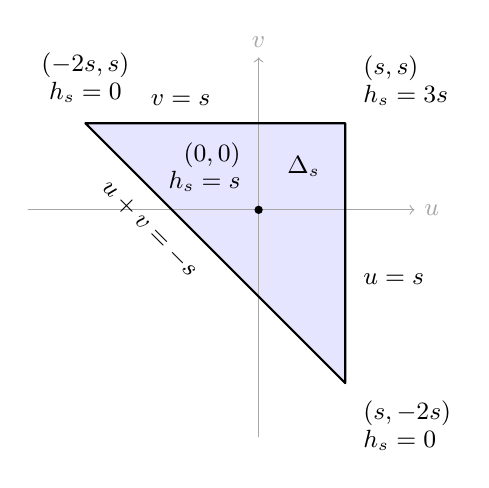
\begin{tikzpicture}[x=1.10cm,y=1.10cm,line cap=round,line join=round,
                      font=\small]
    \fill[blue!10] (-2,1) -- (1,1) -- (1,-2) -- cycle;
    \draw[gray!70,->] (-2.66,0) -- (1.80,0) node[right] {$u$};
    \draw[gray!70,->] (0,-2.62) -- (0,1.76) node[above] {$v$};
    \draw[thick] (-2,1) -- (1,1) -- (1,-2) -- cycle;
    \node[above=4pt,align=center] at (-2,1)
      {$(-2s,s)$\\[-1pt] $h_s=0$};
    \node[above right=3pt,align=left] at (1,1)
      {$(s,s)$\\[-1pt] $h_s=3s$};
    \node[below right=3pt,align=left] at (1,-2)
      {$(s,-2s)$\\[-1pt] $h_s=0$};
    \node[above=3pt] at (-.90,1) {$v=s$};
    \node[right=3pt] at (1,-.80) {$u=s$};
    \node[rotate=-45,below=4pt] at (-1.02,.02) {$u+v=-s$};
    \node at (.52,.50) {$\Delta_s$};
    \fill (0,0) circle[radius=1.5pt];
    \node[above left=3pt,align=right] at (0,0)
      {$(0,0)$\\[-1pt] $h_s=s$};
  \end{tikzpicture}
  \[
    \int_{\Delta_s}h_s(u,v)\,du\,dv
    =\underbrace{\frac{(3s)^2}{2}}_{\text{area}}
      \underbrace{\frac{3s+0+0}{3}}_{\text{mean affine height}}
    =\frac{27s^3}{6}.
  \]
  \caption{For fixed $T=s>0$, the positive integrand is supported,
  within $u\le s$ and $v\le s$, on
  $\Delta_s=\{(u,v):u\le s,\ v\le s,\ s+u+v\ge0\}$.
  Here $h_s(u,v)=s+u+v$ is an affine height, with the displayed values at
  the vertices and barycenter. The shading marks the integration region,
  not the support or density of the Gaussian pair $(U,V)$.
  Multiplying the unweighted integral by the density bound $M$ gives
  the estimate used in the proof. At $s=0$ the triangle degenerates and
  the integral is zero.}
  \label{fig:residual-score-triangle}
\end{figure}

Using \eqref{geo:density-bound},
independence, and $\mathbb E[T_+^3]=2/\sqrt{2\pi}$, we obtain
\[
 Bt<\mathbb E[\mathbf 1_KT]
 \le \frac{27M}{6}\,\mathbb E[T_+^3]
 =\frac{9t^2(1+a_j)(1+a_k)}{2\pi\sqrt{2\pi}\,D_{jk}}.
\]
Since $B=3/(2\sqrt{2\pi})$, this gives
\eqref{geo:pair-bound}, in fact with a strict inequality.
\end{proof}

The pairwise inequality becomes useful for the partition problem when
we sum it over competitors with the largest centroid lengths. The
negative off-diagonal covariances prevent all of these pairwise
determinants from being small simultaneously.

\begin{corollary}[Constraints on the three largest radii]
\label{geo:constraints}
The quantities $L,c,t$ satisfy
\begin{align}
 (c-t^2)(L-c-2t^2)
 &\le8\left(\frac3\pi\right)^2t^2,
 \label{geo:first-constraint}\\
 \frac32(c-t^2)^2
 &\le10\left(\frac3\pi\right)^2t^2.
 \label{geo:second-constraint}
\end{align}
\end{corollary}

\begin{proof}
For the first inequality, the signs and row sums of $H$ give
\[
 H_{31}^2+H_{32}^2
 \le (|H_{31}|+|H_{32}|)^2\le h_3^2.
\]
It follows that
\begin{equation}
 D_{31}^2+D_{32}^2\ge h_3(h_1+h_2-h_3).
 \label{geo:row-lower}
\end{equation}
By \eqref{geo:covariance} and $0<a_j\le1$,
\[
 h_3\ge c-t^2\ge0,
 \qquad h_1+h_2-h_3\ge L-c-2t^2.
\]
If $L-c-2t^2\ge0$, these inequalities and \eqref{geo:row-lower}
show that
\[
 D_{31}^2+D_{32}^2\ge(c-t^2)(L-c-2t^2).
\]
If $L-c-2t^2<0$, the same conclusion follows from the
nonnegativity of the determinant squares.

On the other hand, Lemma~\ref{geo:pair} gives
\[
 D_{31}^2+D_{32}^2
 \le\left(\frac3\pi\right)^2t^2
 (1+a_3)^2\big((1+a_1)^2+(1+a_2)^2\big).
\]
Because $a_1+a_2\le1-a_3$,
\[
 (1+a_1)^2+(1+a_2)^2
 \le (2-a_3)^2+1.
\]
For $0\le x\le1$, the identity
\[
 8-(1+x)^2\big((2-x)^2+1\big)=(1-x)^2(3-x^2)\ge0
\]
therefore proves \eqref{geo:first-constraint}.

For the second inequality, let
$\rho_{jk}=H_{jk}/\sqrt{h_jh_k}$ for $1\le j<k\le3$.
These correlations belong to $[-1,0]$.  Since
\[
 0\le\operatorname{Var}\left(\sum_{j=1}^3\frac{Y_j}{\sqrt{h_j}}\right)
 =3+2\sum_{1\le j<k\le3}\rho_{jk},
\]
we have
\[
 \sum_{j<k\le3}\rho_{jk}^2
 \le\sum_{j<k\le3}|\rho_{jk}|\le\frac32.
\]
Each $h_j\ge c-t^2\ge0$ for $j\le3$.  Thus
\begin{equation}
 \sum_{j<k\le3}D_{jk}^2
 =\sum_{j<k\le3}h_jh_k(1-\rho_{jk}^2)
 \ge\frac32(c-t^2)^2.
 \label{geo:correlation-lower}
\end{equation}
To bound the sum furnished by Lemma~\ref{geo:pair}, put
\[
 s_1=a_1+a_2+a_3,\qquad
 s_2=a_1a_2+a_1a_3+a_2a_3,\qquad s_3=a_1a_2a_3.
\]
Equation~\eqref{geo:coefficients} implies
$0\le s_1\le1$, $0\le s_2\le s_1^2/3\le1/3$, and $s_3\ge0$.
Expanding in these elementary symmetric functions gives
\begin{align*}
 \sum_{j<k\le3}(1+a_j)^2(1+a_k)^2
 &=3+4s_1+2s_1^2+2s_1s_2+s_2^2-(6+2s_1)s_3\\
 &\le3+4+2+\frac23+\frac19=\frac{88}{9}<10.
\end{align*}
Squaring \eqref{geo:pair-bound}, summing over the three pairs, and
combining with \eqref{geo:correlation-lower} proves
\eqref{geo:second-constraint}.
\end{proof}

\section{Excluding five or more active cells}\label{elim:section}

We show that the scalar bounds of Lemma~\ref{sc:bounds} and the
geometric constraints of Corollary~\ref{geo:constraints} are incompatible.
We first confine the smallest radius to $.066<t<.12$, and then prove
$c>2.6t$, contradicting the second determinant constraint.
Throughout this section, the radii are ordered as
\[
 r_1\ge\cdots\ge r_m=t>0,\qquad
 \sum_{j=1}^m r_j^2=1,\qquad
 L=r_1^2+r_2^2,\qquad c=r_3^2.
\]
Set
\begin{equation}\label{elim:parameters}
 A=\begin{cases}.929,&m=5,\\.884,&m\ge6,\end{cases}
 \qquad d=A-.15,\qquad s=\frac{.415}{d},
 \qquad e(u)=.415u-du^2.
\end{equation}
The probability excesses
\(\delta_j=P_j-Ar_j^2\) satisfy, by \eqref{sc:three-bounds},
\begin{equation}\label{elim:budget}
 \delta_j\ge\max\{0,e(r_j)\},\qquad
 \sum_{j=1}^m\delta_j=1-A.
\end{equation}
All terminating decimals below denote exact rational numbers. The finite
comparisons are recorded with strict lower bounds; the rational arithmetic
and square-root enclosures that verify them are described in
Appendix~\ref{cert:arithmetic}.

\subsection{The third radius and the small-minimum case}

First we obtain a bound that holds for every value of~$t$.
For $j\ge3$, the inequality $r_j\le\sqrt c$ gives
\[
 e(r_j)=r_j^2\left(\frac{.415}{r_j}-d\right)
 \ge r_j^2\left(\frac{.415}{\sqrt c}-d\right).
\]
Summing these charges in \eqref{elim:budget} yields
\[
 (1-L)\left(\frac{.415}{\sqrt c}-d\right)\le1-A.
\]
If $A=.929$, add $.045(1-L)$ to both sides and bound the added
right-hand term by $.045$; if $A=.884$, no adjustment is needed. Thus in both cases
\begin{equation}\label{elim:common-charge}
 (1-L)\left(\frac{.415}{\sqrt c}-.734\right)\le.116.
\end{equation}
Since $r_j\le2/3$, we have $L\le8/9$. If $\sqrt c\le.23$,
the left side of \eqref{elim:common-charge} exceeds its right side by
at least
\[
 \frac19\left(\frac{.415}{.23}-.734\right)-.116
 =\frac{101}{34500}>0.
\]
Consequently
\begin{equation}\label{elim:third-radius}
 \sqrt c>.23.
\end{equation}

Suppose now that $t\le q_0:=.066$. We contradict
\eqref{geo:first-constraint}, which reads
\begin{equation}\label{elim:first-constraint}
 (c-t^2)(L-c-2t^2)\le8(3/\pi)^2t^2.
\end{equation}
If $\sqrt c\ge.44$, then $L\ge2c$, so the left side is at least
\[
 (c-t^2)(c-2t^2)
 \ge(.44^2-q_0^2)(.44^2-2q_0^2).
\]
Both factors here are positive, and
\begin{equation}\label{elim:large-third-small-minimum}
 (.44^2-q_0^2)(.44^2-2q_0^2)
       -8(3/\pi)^2q_0^2>.00321132.
\end{equation}
This contradicts \eqref{elim:first-constraint}.

For the remaining range $.23<\sqrt c<.44$, use the four intervals
in Table~\ref{elim:small-table}. On an interval $[a,b]$, the denominator
$.415/\sqrt c-.734$ is positive, and
\eqref{elim:common-charge} gives
\[
 L-c-2t^2
 \ge 1-\frac{.116}{.415/b-.734}-b^2-2q_0^2
 =:M(b).
\]
Also $c-t^2\ge a^2-q_0^2>0$. Every $M(b)$ is positive, and the
last column of the table contradicts \eqref{elim:first-constraint}.
Thus
\begin{equation}\label{elim:minimum-lower}
 t>.066.
\end{equation}

\begin{table}[ht]
\centering
\begin{tabular}{c|c|c}
$[a,b]$ & \shortstack{Lower bound for\\ $M(b)$} &
 \shortstack{Lower bound for\\ $(a^2-q_0^2)M(b)-8(3/\pi)^2q_0^2$}\\
\hline
$[.23,.30]$ & $.72264$ & $.00330237$\\
$[.30,.35]$ & $.61198$ & $.02063552$\\
$[.35,.41]$ & $.40621$ & $.01621418$\\
$[.41,.44]$ & $.24314$ & $.00803616$
\end{tabular}
\caption{Strict lower bounds excluding $t\le.066$ when $\sqrt c<.44$.}
\label{elim:small-table}
\end{table}

\subsection{Bounding the remaining radii}

We next prove that
\begin{equation}\label{elim:tail-cap}
 r_j\le.42\qquad(j\ge4).
\end{equation}
Suppose instead that $r_4>.42$, and put
\[
 K=\frac{d\cdot.42}{s+.42}.
\]
For every $u\ge.42$ we have
\begin{equation}\label{elim:clipped-charge}
 \max\{0,e(u)\}\ge K(s^2-u^2).
\end{equation}
Indeed, when $u\le s$, use
\[
 e(u)=\frac{du}{s+u}(s^2-u^2)
 \quad\hbox{and}\quad \frac{u}{s+u}\ge\frac{.42}{s+.42}.
\]
When $u>s$, the right side of \eqref{elim:clipped-charge} is negative,
so nonnegativity proves the inequality. Applying this to the first four
radii and using the minimum radius on the others gives
\[
 \sum_{j=1}^4\delta_j
 \ge K\left(4s^2-\sum_{j=1}^4r_j^2\right)
 \ge K\bigl(4s^2-1+(m-4)t^2\bigr).
\]
For $j\ge5$, ordering and normalization give
$r_j\le1/\sqrt5$. By \eqref{elim:minimum-lower}, these radii lie
in $[.066,1/\sqrt5]$. Concavity of $e$ therefore gives
\[
 \delta_j\ge\min\{e(.066),e(1/\sqrt5)\}=e(.066).
\]
The last equality follows from Table~\ref{elim:four-table}, where
$e(.066)=.023996676$ for $A=.929$ and
$e(.066)=.024192696$ for $A=.884$.
Combining the charges and replacing $t$ by $.066$ proves
\begin{equation}\label{elim:four-charge}
 1-A\ge K\bigl(4s^2-1+(m-4)(.066)^2\bigr)+(m-4)e(.066).
\end{equation}
The right side increases with $m$, with increment
$K(.066)^2+e(.066)>0$. At the smallest permitted $m$, its excess
over $1-A$ is already positive by Table~\ref{elim:four-table}.
This contradiction proves \eqref{elim:tail-cap}.

\begin{table}[ht]
\centering
\begin{tabular}{c|c|c|c}
$A$ & smallest $m$ & \shortstack{Lower bound for\\ $e(1/\sqrt5)$} &
 \shortstack{Lower bound for the right side of\\ \eqref{elim:four-charge} minus $1-A$}\\
\hline
$.929$ & $5$ & $.02979364$ & $.00092980$\\
$.884$ & $6$ & $.03879364$ & $.02229774$
\end{tabular}
\caption{Strict lower bounds excluding four radii greater than $.42$.}
\label{elim:four-table}
\end{table}

Put $k=2$ when $m=5$ and $k=3$ when $m\ge6$. There are at least
$k$ indices after the first three, and their radii belong to $[t,.42]$.
Their charges are each at least $\min\{e(t),e(.42)\}$. Moreover,
\begin{equation}\label{elim:cap-budget}
 ke(.42)-(1-A)=
 \begin{cases}.0027688,&A=.929,\\.0184672,&A=.884.
 \end{cases}
\end{equation}
Hence \eqref{elim:budget} forces $ke(t)\le1-A$.
Let $t_0$ be the smaller root of $ke(u)=1-A$:
\begin{equation}\label{elim:tzero}
 t_0=\frac{.415-\sqrt{.415^2-4d(1-A)/k}}{2d}.
\end{equation}
Equation~\eqref{elim:cap-budget} places $.42$ strictly between the
two roots of this concave quadratic. Since $t\le.42$, the larger-root
alternative is excluded, and $t\le t_0$. The enclosures
\begin{equation}\label{elim:tzero-enclosures}
 \begin{aligned}
 .1070554<t_0<.1070555&\qquad(A=.929),\\
 .1176565<t_0<.1176566&\qquad(A=.884)
 \end{aligned}
\end{equation}
imply $t_0<.109$ in the first case and $t_0<.12$ in both cases.
Furthermore, $e(.42)>(1-A)/k\ge e(t)$, so each of the $k$ selected
indices contributes at least $e(t)$.

\subsection{The final contradiction}

We claim that
\begin{equation}\label{elim:third-versus-minimum}
 c>2.6t.
\end{equation}
Otherwise, \eqref{elim:third-radius} places the third radius in
$[.23,\sqrt{2.6t}]$. It is distinct from the $k$ indices just charged,
so concavity of $e$ and \eqref{elim:budget} imply
\begin{equation}\label{elim:last-budget}
 1-A\ge\min\{e(.23),e(\sqrt{2.6t})\}+ke(t).
\end{equation}
We check both possible endpoint charges on the entire interval
$[.066,t_0]$.

First, $e$ is increasing up to $t_0$, the smaller root in
\eqref{elim:tzero}. Thus
\[
 e(.23)+ke(t)-(1-A)
 \ge e(.23)+ke(.066)-(1-A)>0,
\]
by Table~\ref{elim:final-table}. Second, the function
\[
 F(t)=e(\sqrt{2.6t})+ke(t)
     =.415\sqrt{2.6t}-2.6dt+k(.415t-dt^2)
\]
is strictly concave for $t>0$, since
\[
 F''(t)=-\frac{.415\sqrt{2.6}}{4t^{3/2}}-2kd<0.
\]
Its minimum on $[.066,t_0]$ is therefore attained at an endpoint.
Table~\ref{elim:final-table} gives $F(.066)>1-A$ and $2.6t_0<s^2$.
The latter implies $e(\sqrt{2.6t_0})>0$; since $ke(t_0)=1-A$, it
also gives $F(t_0)>1-A$. These inequalities contradict
\eqref{elim:last-budget} and prove \eqref{elim:third-versus-minimum}.

\begin{table}[ht]
\centering
\begin{tabular}{c|c|c|c}
$A$ & \shortstack{Exact value of\\ $e(.23)+ke(.066)-(1-A)$} &
 \shortstack{Lower bound for\\ $F(.066)-(1-A)$} &
 \shortstack{Lower bound for\\ $s^2-2.6t_0$}\\
\hline
$.929$ & $.031234252$ & $.01522916$ & $.00546157$\\
$.884$ & $.013199488$ & $.00253590$ & $.01376450$
\end{tabular}
\caption{Positive endpoint margins for \eqref{elim:last-budget}.
The second column is exact; the last two columns give strict lower bounds.}
\label{elim:final-table}
\end{table}

Finally, \eqref{geo:second-constraint}, \eqref{elim:third-versus-minimum},
and $0<t<.12$ give
\[
 10(3/\pi)^2t^2
 \ge1.5(c-t^2)^2
 >1.5(2.6-.12)^2t^2.
\]
But
\[
 1.5(2.6-.12)^2-10(3/\pi)^2>.10667806>0.
\]
This contradiction rules out $C>B^2$ and completes the upper bound.


\begin{proof}[Completion of the proof of Theorem~\ref{thm:main}]
Section~\ref{elim:section} rules out $C>9/(8\pi)$ for the supremum
defined in Section~\ref{ext:section}. The product-and-empty-cell reduction
at the start of that section transfers this bound to every dimension
and finite cell count. The construction in Section~\ref{sec:example}
attains the bound whenever $d\ge2$ and $k\ge3$.
\end{proof}

\subsection{Gaussian maxima}
The partition bound also gives a sharp inequality for Gaussian maxima.
The four-score version appears in Heilman, Jagannath, and
Naor~\cite[Theorem~1.2]{HJN}; Gaussian partition duality is due to
Khot and Naor~\cite[Lemma~3.7]{KhotNaor}. Subtracting the common average
score gives the following centered form in every dimension.

\begin{corollary}[Gaussian maxima]\label{cor:gaussian-maxima}
Let $d,k$ be positive integers, let $g$ be standard Gaussian in
$\mathbb R^d$, and let $v_1,\ldots,v_k\in\mathbb R^d$, with
$\bar v=k^{-1}\sum_{i=1}^k v_i$. Then
\[
 \mathbb E\max_{1\le i\le k}\langle v_i,g\rangle
 \le\frac{3}{2\sqrt{2\pi}}
       \left(\sum_{i=1}^k\|v_i-\bar v\|^2\right)^{1/2}.
\]
The constant is sharp already for three vectors in the plane.
\end{corollary}
\begin{proof}
Put $u_i=v_i-\bar v$. Subtracting the common score
$\langle\bar v,g\rangle$ leaves the expected maximum unchanged.
Partition $\mathbb R^d$ according to the largest score
$\langle u_i,x\rangle$, resolving ties by the smallest index, and let
$z_i$ be the Gaussian first moments of these cells. Then
Theorem~\ref{thm:main} and Cauchy--Schwarz give
\[
 \mathbb E\max_i\langle v_i,g\rangle
 =\sum_i\langle u_i,z_i\rangle
 \le\left(\sum_i\|u_i\|^2\right)^{1/2}
      \left(\sum_i\|z_i\|^2\right)^{1/2}
 \le\frac{3}{2\sqrt{2\pi}}
      \left(\sum_i\|u_i\|^2\right)^{1/2}.
\]
For sharpness, take the three centroid vectors of the planar propeller
in Section~\ref{sec:example}. Their sum is zero, their score cells are
the propeller sectors, and both inequalities are equalities.
\end{proof}

Every finite centered jointly Gaussian vector $(X_1,\ldots,X_k)$ can be
written as $(\langle v_i,g\rangle)_{i=1}^k$, including when its
covariance is singular. Thus the corollary also bounds its expected maximum by
$3/(2\sqrt{2\pi})$ times
$\bigl(\sum_i\operatorname{Var}(X_i-\bar X)\bigr)^{1/2}$, where
$\bar X=k^{-1}\sum_iX_i$.

\section{A kernel-clustering application}\label{kc:section}

\subsection{The objective and the approximation threshold}

This application uses Theorem~\ref{thm:main},
the kernel-clustering results of Khot and Naor, and the companion paper
\emph{The Unique Games Theorem}. None of these complexity arguments is used
in the proof of the Gaussian inequality.

Fix an integer \(k\ge3\). An input is an explicitly represented rational
symmetric matrix \(A=(a_{pq})_{p,q=1}^N\) satisfying
\(A\succeq0\) and \(A\one=0\). The latter is the centering condition;
for a positive semidefinite matrix it is equivalent to
\(\sum_{p,q}a_{pq}=0\). For a map \(\sigma:[N]\to[k]\), define
\begin{equation}\label{kc:value}
 \val_A(\sigma)=\sum_{p,q=1}^N a_{pq}\one_{\{\sigma(p)=\sigma(q)\}},
 \qquad
 \Clust(A\mid I_k)=\max_{\sigma:[N]\to[k]}\val_A(\sigma).
\end{equation}
Here \([m]=\{1,\ldots,m\}\), and \(I_k\) is the \(k\)-by-\(k\)
identity target matrix. The sum is over ordered pairs and includes the
diagonal. Equivalently, it is
\(\sum_{i=1}^k\sum_{p,q\in S_i}a_{pq}\) for the cells
\(S_i=\sigma^{-1}(i)\); empty cells are allowed. There is no
normalization by cell cardinalities. Each objective value is nonnegative,
since it is a sum of quadratic forms \(\one_{S_i}^{\mathsf T}A\one_{S_i}\).

A deterministic approximation with \emph{loss factor} \(\alpha\ge1\)
returns an assignment of value at least
\(\Clust(A\mid I_k)/\alpha\). An expected approximation has the same
inequality with the returned value replaced by its expectation.
Put
\[
 c_*=\frac9{8\pi},
 \qquad
 \alpha_k=\frac{1-1/k}{c_*}
          =\frac{8\pi}{9}\left(1-\frac1k\right).
\]

\paragraph{The matching rounding constant.}
Khot and Naor's approximation theorem
\cite[Theorem~2.1]{KhotNaor}
gives the expected rounding bound
\[
 \E\val_A(\sigma)\ge\frac{\Clust(A\mid I_k)}{\alpha_k}
\]
on the inputs in \eqref{kc:value}. This is their endpoint analytic
guarantee using an optimal semidefinite relaxation and ideal Gaussian
sampling. We quote this rounding guarantee separately from the
rational-input hardness statement below; an exact finite-bit
implementation at the endpoint is not asserted here.

\begin{theorem}[Kernel-clustering hardness]\label{kc:main}
For each fixed \(k\ge3\) and every fixed
\(1\le\alpha<\alpha_k\), it is NP-hard, given a rational symmetric
matrix \(A\succeq0\) with \(A\one=0\) and the identity-target
objective \eqref{kc:value}, to find
\(\sigma:[N]\to[k]\) such that
\[
 \val_A(\sigma)\ge\Clust(A\mid I_k)/\alpha.
\]
In particular, such a deterministic polynomial-time approximation
would imply \(\mathrm P=\mathrm{NP}\).
\end{theorem}

We prove the hardness statement below. It concerns strict improvement
over \(\alpha_k\), not hardness at the endpoint.

For the more general objective $\sum_{p,q}a_{pq}b_{\sigma(p)\sigma(q)}$
with a fixed positive semidefinite target matrix $B=(b_{ij})_{i,j=1}^k$,
Khot and Naor later characterized the Unique Games hardness threshold
for approximating the optimal clustering value through geometric and
Gaussian partition parameters
\cite[Theorem~1.1]{KhotNaorSharp}. Here the target is $I_k$, and the
Gaussian constant is supplied by Theorem~\ref{thm:main}.

\subsection{The two external hardness inputs}

The Gaussian parameter in Khot and Naor's theorem is
\[
 C_k:=\sup_{(B_1,\ldots,B_k)}
 \sum_{i=1}^k
 \left\|\int_{B_i}x\,d\gamma_{k-1}(x)\right\|^2.
\]
The supremum ranges over measurable partitions of \(\R^{k-1}\),
with empty cells allowed. Since \(k\ge3\),
Theorem~\ref{thm:main} and the attaining example in
Section~\ref{sec:example} give
\begin{equation}\label{kc:gaussian-constant}
 C_k=c_*.
\end{equation}

We first specify the discrete analytic input. Let \(\Omega=[k]\) have
uniform probability measure. Choose a real orthonormal basis
\(b_0,b_1,\ldots,b_{k-1}\) of functions on \(\Omega\), with \(b_0=1\).
For \(r\in\N\) and \(\nu\in\{0,\ldots,k-1\}^r\), write
\[
 b_\nu(x)=\prod_{j=1}^r b_{\nu_j}(x_j),
 \qquad
 |\nu|=\bigl|\{j:\nu_j\ne0\}\bigr|.
\]
Every \(h:\Omega^r\to\R\) has expansion
\(h=\sum_\nu\widehat h(\nu)b_\nu\), with coefficients computed using
uniform probability measure. For real \(D\ge0\), set
\begin{equation}\label{kc:influence}
 \Inf_j^{\le D}(h)=
 \sum_{\substack{|\nu|\le D\\\nu_j\ne0}}\widehat h(\nu)^2.
\end{equation}
Thus a nonintegral cutoff is interpreted by the displayed inequality
on the integer \(|\nu|\). Let \(P_1\) be orthogonal projection onto
the span of \(b_\nu\) with \(|\nu|=1\), and, for
\(f=(f_1,\ldots,f_k)\), put
\[
 \OBJ(f)=\sum_{i=1}^k\|P_1f_i\|_2^2.
\]
All \(L_2\) norms in this section use uniform probability measure.
Define the closed simplex with slack by
\[
 \Delta_k=\{u\in\R^k:u_i\ge0,\ \sum_{i=1}^k u_i\le1\}.
\]

\begin{theorem}[Khot--Naor low-influence bound]\label{kc:kn-input}
For fixed \(k\) and every \(\eta>0\), there exists \(0<\tau_0<1/2\),
independent of \(r\), such that every \(r\in\N\) and every
\(f:\Omega^r\to\Delta_k\) satisfying
\[
 \Inf_j^{\le\log(1/\tau_0)}(f_i)\le\tau_0
 \quad(i\in[k],\ j\in[r])
\]
obey \(\OBJ(f)\le C_k+\eta\).
\end{theorem}

This is \cite[Theorem~3.8]{KhotNaor}, with the same uniform product
measure, Fourier degree, simplex, and Gaussian normalization. Its proof
uses the invariance principle of Mossel, O'Donnell, and
Oleszkiewicz~\cite{MOO} to compare low-influence functions on product
spaces with their Gaussian counterparts.
The restriction \(\tau_0<1/2\) is harmless: decreasing the threshold
and increasing the degree cutoff strengthen the hypotheses.
Choose a rational \(0<\tau<\min\{\tau_0,1/2\}\) and set
\begin{equation}\label{kc:cutoff}
 D=\max\{1,\lceil\log(1/\tau)\rceil\}.
\end{equation}
Monotonicity of \eqref{kc:influence} in the cutoff gives the useful
contrapositive
\begin{equation}\label{kc:contrapositive}
 \OBJ(f)>C_k+\eta
 \quad\Longrightarrow\quad
 \Inf_j^{\le D}(f_i)>\tau
 \text{ for some }i\in[k],\ j\in[r].
\end{equation}
Indeed, if every influence at cutoff \(D\) were at most \(\tau\),
every influence at the original cutoff would be at most \(\tau_0\).

The second input is the following exact interface of
\cite[Theorem~1.1]{UniqueGamesTheorem}.

\begin{theorem}[Unique Games input]\label{kc:ug-input}
For every fixed \(\varepsilon,\delta\in(0,1/2)\), there are an
integer \(s\ge1\) and a deterministic polynomial-time reduction
from \(\mathrm{3SAT}\) to explicit unweighted simple bipartite
Unique Games instances over \(\mathbb F_2^s\). If the formula is
satisfiable the game has a labeling satisfying at least
\(1-\varepsilon\) of its edges; if it is unsatisfiable every
labeling satisfies at most \(\delta\) of its edges. The edge set
is nonempty and each constraint is a translation of the alphabet.
The alphabet size and the polynomial's degree and constants depend
only on \(\varepsilon,\delta\).
\end{theorem}

Only ordinary satisfied-edge fractions are asserted here. We will
use neither regularity nor the stronger condition that almost every
left vertex has all its incident constraints satisfied.

\subsection{A rational centered positive semidefinite matrix}

Let \(G=(V,W,E)\) be a game supplied by
Theorem~\ref{kc:ug-input}, and enumerate its alphabet as
\([r]\), where \(r=2^s\). Reorient constraints if necessary so that
the permutation \(\pi_{vw}:[r]\to[r]\) attached to \(vw\in E\)
is satisfied precisely when
\[
 \ell(v)=\pi_{vw}(\ell(w)).
\]
Translations are permutations, so this changes no game value.
Delete isolated vertices, put \(M=|E|\), and write
\[
 d_v=|N(v)|,\qquad \mu(v)=\frac{d_v}{M}\quad(v\in V).
\]
Choosing \(v\) with probability \(\mu(v)\), then a uniform
\(w\in N(v)\), chooses an edge uniformly.

To fix the permutation convention, for a permutation \(\pi\) define
\[
 (R_\pi x)_a=x_{\pi(a)}\quad(a\in[r]).
\]
For a scalar table \(h:W\times\Omega^r\to\R\), define
\begin{equation}\label{kc:averaging}
 (T_vh)(x)=\frac1{d_v}
       \sum_{w\in N(v)}h(w,R_{\pi_{vw}}x),
 \qquad
 Q(h)=\sum_{v\in V}\mu(v)\|P_1T_vh\|_2^2 .
\end{equation}
The output matrix will represent \(Q\) in the ordinary,
unnormalized Euclidean coordinates of the table \(h\).

\begin{lemma}\label{kc:matrix}
For fixed \(k,r\), one can construct in deterministic polynomial
time a rational symmetric matrix \(A\), indexed by
\(W\times\Omega^r\), such that
\[
 h^{\mathsf T}Ah=Q(h),\qquad A\succeq0,\qquad A\one=0 .
\]
For every \(\sigma:W\times\Omega^r\to[k]\), if
\(F_i(w,x)=\one_{\{\sigma(w,x)=i\}}\), then
\begin{equation}\label{kc:objective-identity}
 \val_A(\sigma)=
 \sum_{v\in V}\mu(v)\OBJ(F_v),\qquad
 F_v=(T_vF_1,\ldots,T_vF_k):\Omega^r\to\Delta_k.
\end{equation}
All output assignment values lie in \([0,1]\).
\end{lemma}

\begin{proof}
Put \(q=k^r\). The projection \(P_1\), written as a matrix acting
on the counting-coordinate vector \((h(x))_{x\in\Omega^r}\), is
\begin{equation}\label{kc:projection-matrix}
 (P_1)_{x,y}=\frac1q
       \sum_{j=1}^r\bigl(k\one_{\{x_j=y_j\}}-1\bigr).
\end{equation}
To see this, the centered subspaces of functions of distinct
individual coordinates are mutually orthogonal. Hence
\[
 (P_1h)(x)=
 \sum_{j=1}^r\bigl(\E[h(X)\mid X_j=x_j]-\E h(X)\bigr),
\]
which is \eqref{kc:projection-matrix}.
This matrix is rational, symmetric and idempotent.
The counting-coordinate matrix of \(T_v\) has entries
\[
 (T_v)_{x,(w,y)}
 =\frac1{d_v}\one_{\{w\in N(v)\}}
           \one_{\{y=R_{\pi_{vw}}x\}} .
\]
Define
\begin{equation}\label{kc:matrix-formula}
 A=\frac1q\sum_{v\in V}\mu(v)T_v^{\mathsf T}P_1T_v.
\end{equation}
There are two factors \(q^{-1}\): one in
\eqref{kc:projection-matrix}, and one outside the sum in
\eqref{kc:matrix-formula} because \(L_2\) uses probability
measure. Symmetry and \(P_1^2=P_1\) give
\[
 h^{\mathsf T}Ah
 =\sum_v\mu(v)\frac1q\|P_1T_vh\|_{\ell_2}^2=Q(h)\ge0.
\]
Also \(T_v\one=\one\) and \(P_1\one=0\), so
\eqref{kc:matrix-formula} gives \(A\one=0\).

There are \(N=|W|k^r\) output indices. For fixed \(k,r\) this is
polynomial in the explicit game size, and the dense matrix can be
computed by rational arithmetic in polynomial time. Its entries
are sums of terms with denominators dividing
\(M d_v q^2\). A common denominator divides
\(M q^2\prod_{v\in V}d_v\), whose bit length is
\(O(\log M+\sum_v\log d_v+\log q)\), and the numerators also
have polynomial bit length. No irrational Fourier basis needs
to be constructed.

By definition of the ordered sum,
\(\val_A(\sigma)=\sum_iF_i^{\mathsf T}AF_i\); inserting
\eqref{kc:averaging} proves \eqref{kc:objective-identity}.
Every \(F_v(x)\) is an average of coordinate unit vectors, so
its entries are nonnegative and sum to one. Parseval and
orthogonal projection give
\begin{equation}\label{kc:objective-bound}
 0\le\OBJ(F_v)
 \le\sum_{i=1}^k\|F_{v,i}\|_2^2
 \le\E\sum_{i=1}^k F_{v,i}=1.
\end{equation}
Since \(\sum_v\mu(v)=1\), the last claim follows.
\end{proof}

\subsection{Completeness and weighted decoding}

The next two lemmas compare ordinary edge-value completeness and
soundness with the kernel objective. They adapt the
Khot--Naor reduction \cite[Section~3.3]{KhotNaor} to the precise
input of Theorem~\ref{kc:ug-input}.

\begin{lemma}[Completeness]\label{kc:completeness}
If a labeling of \(G\) satisfies at least \(1-\varepsilon\) of
its edges, then the matrix of Lemma~\ref{kc:matrix} satisfies
\[
 \Clust(A\mid I_k)\ge
       \left(1-\frac1k\right)(1-\varepsilon)^2.
\]
\end{lemma}
\begin{proof}
Use a witnessing labeling \(\ell\) to set
\(\sigma(w,x)=x_{\ell(w)}\).
For \(j\in[r]\), let \(D_j(x)=e_{x_j}\), where
\(e_1,\ldots,e_k\) are the coordinate unit vectors in \(\R^k\).
With
\[
 p_{v,j}=
 \Pr_{w\in N(v)}\{\pi_{vw}(\ell(w))=j\},
\]
the chosen permutation convention gives
\(F_v=\sum_{j=1}^r p_{v,j}D_j\).
For each \(i\), the level-one part of the \(i\)-th component of
\(D_j\) is \(\one_{\{x_j=i\}}-1/k\). These parts for different
\(j\)'s are orthogonal. Moreover,
\[
 \sum_{i=1}^k
 \E\bigl(\one_{\{X_j=i\}}-1/k\bigr)^2=1-\frac1k.
\]
It follows that
\[
 \OBJ(F_v)=
 \left(1-\frac1k\right)\sum_{j=1}^r p_{v,j}^2
 \ge \left(1-\frac1k\right)p_{v,\ell(v)}^2.
\]
The weighted mean \(\E_{v\sim\mu}p_{v,\ell(v)}\) is exactly
the satisfied-edge fraction of \(\ell\), and is therefore at
least \(1-\varepsilon\). Jensen's inequality and
\eqref{kc:objective-identity} prove the claim.
\end{proof}

\begin{lemma}[Soundness]\label{kc:soundness}
Fix \(\eta>0\) with \(C_k+2\eta<1\), and choose
\(\tau,D\) as in \eqref{kc:cutoff} for this \(\eta\).
If every labeling of \(G\) satisfies at most \(\delta\) of its
edges, where
\begin{equation}\label{kc:delta}
 0<\delta<\frac{\eta\tau^2}{4kD},
\end{equation}
then
\(\Clust(A\mid I_k)\le C_k+2\eta\).
\end{lemma}
\begin{proof}
Suppose an assignment \(\sigma\) gives a larger value, and use
the functions in Lemma~\ref{kc:matrix}.
Let
\[
 V_{\mathrm{good}}=
       \{v:\OBJ(F_v)>C_k+\eta\}.
\]
If its \(\mu\)-mass is \(\beta\), then
\eqref{kc:objective-bound} gives
\[
 \sum_v\mu(v)\OBJ(F_v)
 \le\beta+(1-\beta)(C_k+\eta)
 \le C_k+\eta+\beta.
\]
The assumed objective therefore forces \(\beta>\eta\).

For every \(v\in V_{\mathrm{good}}\),
\eqref{kc:contrapositive} supplies
\(i_v\in[k]\) and \(j_v\in[r]\) with
\(\Inf_{j_v}^{\le D}(F_{v,i_v})>\tau\).
Taking the squared norm of the relevant Fourier coefficients
in the neighbor average, and using convexity, gives
\begin{equation}\label{kc:influence-average}
 \Inf_{j_v}^{\le D}(F_{v,i_v})
 \le \frac1{d_v}\sum_{w\in N(v)}
       \Inf_{\pi_{vw}^{-1}(j_v)}^{\le D}(F_{i_v}(w,\cdot)).
\end{equation}
The inverse permutation in this formula follows directly from
\((R_\pi x)_a=x_{\pi(a)}\): the Fourier indices involving
left coordinate \(j_v\) come from right coordinate
\(\pi^{-1}(j_v)\).
Every influence on the right belongs to \([0,1]\), by
Parseval and \(0\le F_i(w,\cdot)\le1\).
An average exceeding \(\tau\) has more than a \(\tau/2\)
fraction of its entries at least \(\tau/2\):
otherwise its average is at most
\(\tau/2+(\tau/2)\cdot1\le\tau\).

For each \(w\in W\), form the finite label list
\[
 L(w)=
 \{a\in[r]:\Inf_a^{\le D}(F_i(w,\cdot))\ge\tau/2
                      \text{ for some }i\in[k]\}.
\]
For every scalar \(h\), counting how often a Fourier coefficient
contributes gives
\[
 \sum_{a=1}^r\Inf_a^{\le D}(h)
 =\sum_{|\nu|\le D}|\nu|\,\widehat h(\nu)^2
 \le D\|h\|_2^2.
\]
Consequently
\begin{equation}\label{kc:list-size}
 |L(w)|\frac{\tau}{2}
 \le\sum_{i=1}^k\sum_{a=1}^r
            \Inf_a^{\le D}(F_i(w,\cdot))
 \le kD,
 \qquad |L(w)|\le\frac{2kD}{\tau}.
\end{equation}

Label a good \(v\) by \(j_v\), and other left vertices arbitrarily.
Independently label each right vertex uniformly from \(L(w)\)
when this list is nonempty, and arbitrarily otherwise.
For a good \(v\), more than a \(\tau/2\) fraction of its
neighbors have \(\pi_{vw}^{-1}(j_v)\in L(w)\), by
\eqref{kc:influence-average}. On each such edge the random label
at \(w\) satisfies the constraint with probability at least
\(\tau/(2kD)\), by \eqref{kc:list-size}.
The expected fraction of satisfied edges is therefore greater than
\[
 \eta\cdot\frac{\tau}{2}\cdot\frac{\tau}{2kD}
   =\frac{\eta\tau^2}{4kD}.
\]
Here the weights \(\mu(v)=d_v/M\) ensure that this is the
uniform-edge fraction. Some deterministic labeling attains at
least its expectation, contradicting \eqref{kc:delta}.
\end{proof}

\subsection{Completing the reduction}

\begin{proof}[Proof of the hardness assertion in Theorem~\ref{kc:main}]
Fix \(k\ge3\) and \(1\le\alpha<\alpha_k\).
First choose rational \(\varepsilon,\eta>0\) sufficiently small
that \(\varepsilon<1/2\), \(c_*+2\eta<1\), and
\begin{equation}\label{kc:separated-gap}
 \alpha<
 \frac{(1-1/k)(1-\varepsilon)^2}{c_*+2\eta}.
\end{equation}
Next choose \(\tau,D\) from Theorem~\ref{kc:kn-input} and
\eqref{kc:cutoff}; these depend on \(k,\eta\), not the game size.
Choose a rational
\[
 0<\delta<
 \min\left\{\frac12,\frac{\eta\tau^2}{4kD}\right\}.
\]
Apply Theorem~\ref{kc:ug-input} with these fixed errors.
Only at this stage is the fixed alphabet size \(r=2^s\)
determined. In particular \(k^r\) is a constant with respect to
the input formula size, although no uniform bound polynomial in
the error reciprocals is asserted.

Compose that deterministic reduction with Lemma~\ref{kc:matrix}.
Lemmas~\ref{kc:completeness} and \ref{kc:soundness}, together with
\eqref{kc:gaussian-constant}, give the gap
\[
 \begin{aligned}
 \varphi\text{ satisfiable}
 &\ \Longrightarrow\
 \Clust(A_\varphi\mid I_k)\ge
       H:=(1-1/k)(1-\varepsilon)^2,\\
 \varphi\text{ unsatisfiable}
 &\ \Longrightarrow\
 \Clust(A_\varphi\mid I_k)\le
       S:=c_*+2\eta .
 \end{aligned}
\]
The output is a rational symmetric centered PSD matrix with
polynomial dimension and bit length. By \eqref{kc:separated-gap},
\(S<H/\alpha\). Choose a fixed rational
\(\theta\) strictly between these numbers.
A deterministic loss-factor-\(\alpha\) algorithm produces value
greater than \(\theta\) on satisfiable formulas; every assignment
has value less than \(\theta\) on unsatisfiable formulas.
The returned value is an exactly computable rational number.
This would decide \(\mathrm{3SAT}\) in polynomial time.
Thus achieving the stated factor is NP-hard.
\end{proof}

\begin{remark}[Randomized guarantees]\label{kc:randomized}
The quoted Khot--Naor rounding guarantee is in expectation.
The deterministic hardness conclusion of Theorem~\ref{kc:main} does
not use \(\mathrm P\ne\mathrm{NP}\) to exclude randomized
algorithms. More precisely, a polynomial-time randomized algorithm
whose expected value is at least \(\Clust(A\mid I_k)/\alpha\)
for some fixed \(\alpha<\alpha_k\) would place
\(\mathrm{3SAT}\) in \(\mathrm{RP}\).
Indeed, on the reduction instances its returned value \(X\) lies
in \([0,1]\). In the satisfiable case \(\E X\ge H/\alpha>\theta\);
therefore
\[
 \Pr\{X>\theta\}\ge
 \frac{H/\alpha-\theta}{1-\theta}>0.
\]
This is a fixed positive constant. In the unsatisfiable case
\(X\le S<\theta\) always. A fixed number of repetitions gives
one-sided success probability at least \(1/2\).
\end{remark}

\begin{remark}[Inputs to the application]\label{kc:dependencies}
The Gaussian proof supplies only \eqref{kc:gaussian-constant}.
Khot and Naor supply the expected rounding guarantee
\cite[Theorem~2.1]{KhotNaor} and the analytic
low-influence bound \cite[Theorem~3.8]{KhotNaor}.
Their reduction in Section~3.3 is the model for
Lemmas~\ref{kc:matrix}--\ref{kc:soundness}; the degree weights and
the squared completeness loss explicitly accommodate the ordinary
edge-value, possibly nonregular instances from
\cite[Theorem~1.1]{UniqueGamesTheorem}.
No stronger Unique Games promise is assumed.
The separate Unique Games theorem is a formal dependency only
of this hardness application. The algorithmic endpoint is quoted
in its ideal rounding formulation; this section supplies no
finite-precision endpoint implementation.
\end{remark}



\appendix
\section{Elementary certificates for the numerical inequalities}
\label{cert:arithmetic}
This appendix gives rational enclosures for the numerical comparisons
used in the proof. All finite decimals denote exact rationals. The
formulas below and the tables suffice to reproduce the comparisons;
no numerical optimization or numerical quadrature is needed.

\subsection{Enclosure formulas}
We use
\begin{equation}\label{cert:pi}
 3.14159<\pi<3.14160.
\end{equation}
For example, these bounds follow from
\(\pi=16\arctan(1/5)-4\arctan(1/239)\) by bounding each arctangent
between its alternating-series partial sums through indices 7 and 6.
All square-root enclosures may be obtained using rational numbers
\(l,u\ge0\) with \(l^2\le x\le u^2\).
An explicit rule, if desired, is to set \(D=10^{35}\) and use
\[
 \frac{\lfloor\sqrt{\lfloor xD^2\rfloor}\rfloor}{D}
 \le\sqrt{x}\le
 \frac{\lfloor\sqrt{\lfloor xD^2\rfloor}\rfloor+1}{D}.
\]
For an interval of possible \(x\), apply the lower rule to its lower
endpoint and the upper rule to its upper endpoint. Thus only rational
operations and integer square roots are required.

For \(y\ge0\), let
\[
 E_N(y)=\sum_{j=0}^N\frac{(-y)^j}{j!}.
\]
Taylor's integral remainder gives
\begin{equation}\label{cert:exponential}
 E_{15}(y)\le e^{-y}\le E_{14}(y).
\end{equation}
This conclusion does not require the initial terms of the series to
be decreasing. Integrating the same bounds, set
\[
 J_N(x)=\sum_{j=0}^N
 \frac{(-1)^j x^{2j+1}}{2^j j!(2j+1)},\qquad x\ge0.
\]
Then
\begin{equation}\label{cert:normal}
 \frac12+\frac{J_{15}(x)}{\sqrt{2\pi}}
 \le\Phi(x)\le
 \frac12+\frac{J_{14}(x)}{\sqrt{2\pi}},\qquad
 \Phi(-x)=1-\Phi(x).
\end{equation}
Together with \eqref{cert:pi} and the square-root rule, these are
rational enclosures for both \(\phi\) and \(\Phi\) at every argument
used below. Interval addition, subtraction, multiplication, and
division by intervals avoiding zero preserve the enclosures.

For the cap calculation, put
\[
 Q(x)=\sum_{j=0}^4\frac{\binom{2j}{j}}{4^j(2j+1)}x^{2j+1}.
\]
The binomial series has positive coefficients at most one. Its tail
starting in degree 10 is bounded by \(x^{10}/(1-x^2)\); after
integration this gives, for \(0\le x<1\),
\begin{equation}\label{cert:arcsine}
 Q(x)\le\arcsin x\le Q(x)+\frac{x^{11}}{11(1-x^2)}.
\end{equation}

\subsection{The two rearrangement minima}
Write \(f(x)=(9/4)e^{x^2}\Phi(-x)\) and
\(D_f(x)=2x-\phi(x)/\Phi(-x)\), as in
\eqref{sc:halfspace-ratio}. Substitution into
\eqref{cert:exponential}--\eqref{cert:normal} gives the following
strict enclosures:
\[
\begin{array}{rcl}
 -0.000131&<&D_f(0.6119)<-0.000126,\\
  0.000120&<&D_f(0.6121)< 0.000124,\\
 -0.000430&<&D_f(x)<0.000424
               \quad(0.6119\le x\le0.6121),\\
  0.884383832&<&f(0.612).
\end{array}
\]
For the third row, use the whole rational interval
\([0.6119,0.6121]\) in the elementary interval operations;
\(\phi(x)\) decreases and \(\Phi(-x)\) decreases there, so endpoint
enclosures give both factors. Thus \(|D_f|<0.001\) throughout that
interval. The minimizer lies within \(0.0001\) of \(0.612\), and so
\[
 \min f\ge f(0.612)e^{-10^{-7}}
 >0.884383832(1-10^{-7})>0.8843837.
\]

For \(p,F,H,R\) from \eqref{sc:cap-ratio} and its following
calculation, \eqref{cert:arcsine} gives
\[
\begin{array}{rcl}
 -0.0047010&<&F(0.29)<-0.0046981,\\
  0.0007683&<&F(0.294)<0.0007712,\\
  0.9312526&<&R(0.29),\\
  0.22198&<&p(0.294)-0.294/\pi.
\end{array}
\]
For \(0.29\le x\le0.294\), the last row implies
\[
 H(x)=p(x)-\frac{x\sqrt{1-x^2}}\pi
 \ge p(0.294)-\frac{0.294}\pi>0.
\]
Therefore \(F\) is increasing throughout the interval, and the first
two rows imply \(|F(x)|<0.004702\) there. Consequently
\[
 |R'(x)|<\frac{(9/4)0.004702}{(1-0.294^2)^4}
 <0.015189<0.03.
\]
This proves the derivative bound on the entire interval. The minimum
therefore exceeds \(0.9312526-0.03(0.004)=0.9311326\).

\subsection{Quantiles and the interval probability bounds}
For \(P_0(a)=(0.415+0.15a)a\), Table~\ref{cert:quantiles}
gives a rational \(q_a\) satisfying \(\Phi(q_a)<P_0(a)\), and a
strict upper bound on \(G(q_a)\). Each entry follows by substituting
the displayed rational argument into
\eqref{cert:exponential}--\eqref{cert:normal} and the definition of
\(G\). Since \(G\) is nonincreasing,
\[
 G\bigl(\Phi^{-1}(P_0(r))\bigr)\le G(q_a)
 \qquad(r\ge a).
\]
In each row the listed upper bound is strictly below the value of
\(U\) in Table~\ref{sc:interval-table}.

\begin{table}[ht]
\centering
\begin{tabular}{rrrr}
\hline
\(a\)&\(q_a\)&\(10^6(P_0(a)-\Phi(q_a))>\)&\(G(q_a)<\)\\
\hline
0.05&-2.033&98&0.887728\\
0.14&-1.548&228&0.854397\\
0.24&-1.238&381&0.826606\\
0.33&-1.024&366&0.803691\\
0.41&-0.860&470&0.783737\\
0.48&-0.728&452&0.766006\\
0.54&-0.621&539&0.750456\\
0.59&-0.535&739&0.737150\\
0.64&-0.450&684&0.723262\\
\hline
\end{tabular}
\caption{Rational enclosures certifying the quantile and \(G\) bounds.}
\label{cert:quantiles}
\end{table}

Finally, for each row \((a,b,U)\) of
Table~\ref{sc:interval-table}, replace \(\pi\) by its upper bound in
\(B^2=9/(8\pi)\), enclose \(\sqrt{1-a^2}\) from above, and subtract
the exact rational \(U(0.415+0.15b)^2\). This gives the lower bounds
in that table's last column. The same rational and square-root rules
apply to the finite comparisons in the numerical elimination section.


\begin{thebibliography}{99}

\bibitem{Borell}
C.~Borell,
\emph{The Ehrhard inequality},
C. R. Acad. Sci. Paris, S\'er. I \textbf{337} (2003), no.~10, 663--666.
\href{https://doi.org/10.1016/j.crma.2003.09.031}{doi:10.1016/j.crma.2003.09.031}.

\bibitem{Ehrhard}
A.~Ehrhard,
\emph{Sym\'etrisation dans l'espace de Gauss},
Math. Scand. \textbf{53} (1983), 281--301.
\href{https://doi.org/10.7146/math.scand.a-12035}{doi:10.7146/math.scand.a-12035}.

\bibitem{HeilmanHyper}
S.~Heilman,
\emph{Hyperstable sets with voting and algorithmic hardness applications},
preprint (2022),
\href{https://arxiv.org/abs/2209.11216v1}{arXiv:2209.11216v1}.

\bibitem{HJN}
S.~Heilman, A.~Jagannath, and A.~Naor,
\emph{Solution of the Propeller Conjecture in $\mathbb R^3$},
Discrete Comput. Geom. \textbf{50} (2013), no.~2, 263--305.
\href{https://doi.org/10.1007/s00454-013-9530-0}{doi:10.1007/s00454-013-9530-0}.

\bibitem{KhotNaor}
S.~Khot and A.~Naor,
\emph{Approximate kernel clustering},
Mathematika \textbf{55} (2009), no.~1--2, 129--165.
\href{https://doi.org/10.1112/S002557930000098X}{doi:10.1112/S002557930000098X}.

\bibitem{KhotNaorSharp}
S.~Khot and A.~Naor,
\emph{Sharp kernel clustering algorithms and their associated
Grothendieck inequalities},
Random Structures Algorithms \textbf{42} (2013), no.~3, 269--300.
\href{https://doi.org/10.1002/rsa.20398}{doi:10.1002/rsa.20398}.

\bibitem{Latala}
R.~Lata\l a,
\emph{A note on the Ehrhard inequality},
Studia Math. \textbf{118} (1996), no.~2, 169--174.
\href{https://doi.org/10.4064/sm-118-2-169-174}{doi:10.4064/sm-118-2-169-174}.

\bibitem{MOO}
E.~Mossel, R.~O'Donnell, and K.~Oleszkiewicz,
\emph{Noise stability of functions with low influences:
Invariance and optimality},
Ann. of Math. (2) \textbf{171} (2010), no.~1, 295--341.
\href{https://doi.org/10.4007/annals.2010.171.295}{doi:10.4007/annals.2010.171.295}.

\bibitem{UniqueGamesTheorem}
OpenAI,
\emph{The Unique Games Theorem},
OpenAI Math Release preprint
\href{https://github.com/openai/math/blob/main/preprints/The-Unique-Games-Theorem-September-23-2026/paper.pdf}{OAI:The-Unique-Games-Theorem-September-23-2026},
2026.
Theorem~1.1.

\bibitem{vanHandel}
R.~van Handel,
\emph{The Borell--Ehrhard game},
Probab. Theory Related Fields \textbf{170} (2018), 555--585.
\href{https://doi.org/10.1007/s00440-017-0762-4}{doi:10.1007/s00440-017-0762-4}.

\end{thebibliography}

\end{document}
